\chapter{Overview}

The \cernvmfs\ (\cvmfs) is a read-only file system designed to deliver high energy physics (HEP) experiment analysis software onto virtual machines and grid worker nodes in a fast, scalable, and reliable way.
%\cvmfs\ decouples the underlying operating system from the experiment defined software stack.
Files and file metadata are downloaded on demand and aggressively cached.
For the distribution of files, \cvmfs\ uses a standard HTTP transport, which allows exploitation of a variety of web caches, including commercial content delivery networks.
\cvmfs\ ensures data authenticity and integrity over these possibly untrusted caches and connections. %while keeping all distributed data cacheable.

The \cvmfs\ software comprises client-side software to mount ``\cvmfs\ repositories'' (similar to AFS volumes) as well as a server-side toolkit to create such distributable \cvmfs\ repositories.
Figure~\ref{fig:concept} shows an overview of software distribution with \cvmfs.
Figure~\ref{fig:fuse} shows how \cvmfs\ interlocks with Fuse and a web server in order to deliver files.

The first implementation of \cvmfs\ was based on \product{grow-fs}~\cite{parrot05, growfs09}, which was originally provided as one of the private file system options available in \indexed{Parrot}. 
Parrot traps the system I/O calls and that is resulting in a performance penalty and occasional compatibility problems with some applications. 
The principal differences of \cvmfs\ compared to \product{grow-fs} are:
\begin{itemize}
	\item Use of the the Fuse kernel module~\cite{fuse} that comes with in-kernel caching of file data and file attributes
	\item Use of a content addressable storage format resulting in immutable files and automatic file de-duplication
	\item Possibility to split a directory hierarchy into sub catalogues at user-defined levels
	\item Automatic updates of file catalogs controlled by a \indexed{time to live}\index{TTL|see{time to live}} stored inside file catalogs
	\item Digitally signed repositories
	\item Transparent file compression/decompression and transparent file chunking
	\item Capability to work in \indexed{offline mode} providing that all required files are cached
	\item File system versioning
	\item File system hotpatching
	\item Dynamical expansion of environment variables embedded in \indexed{symbolic link}s\index{symlink|see{symbolic link}}
	\item Automatic server selection
	\item Automatic load-balancing of proxy servers
	\item Support for WPAD/PAC auto-configuration of proxy servers
	\item Efficient replication of repositories
	\item Possibility to use a key-value store instead of a file system as repository storage
\end{itemize}

%\cvmfs\ can be seen as network file system (Figure~\ref{fig:classification}).
%Though the task of installing software is done remotely on the repository side, software is still executed locally under control of the user.
%This is in contrast to software as a service where control is completely handed over to a third party.
In contrast to general purpose network file systems such as \nfs\ or \afs, \cvmfs\ is particularly crafted for fast and scalable software distribution.
Running and compiling software that is hosted on shared areas is typically hard for general purpose network file systems.
%For instance, running and compiling software might easily overload \nfs\ or \product{Lustre}~\cite{lustre03} shared software areas.

In order to create and update a \cvmfs\ repository, a distinguished machine, the so-called \emph{Release Manager Machine}, is used.
On such a release manager machine, a \cvmfs\ repository is mounted in read/write mode by means of a union file system~\cite{unionfs04}.
The union file system overlays the \cvmfs\ read-only mount point by a writable scratch area.
The \cvmfs\ server tool kit merges changes written to the scratch area into the \cvmfs\ repository.
Merging and publishing changes can be triggered at user-defined points in time; it is an atomic operation.
As such, a \cvmfs\ repository is similar to a repository in the sense of a versioning system.

\begin{figure}
	\begin{center}
		\resizebox{\textwidth}{!}{%\documentclass[a4paper, 11pt]{article}\usepackage{tikz,ifthen}\usetikzlibrary{arrows,positioning,shapes,topaths,calc,fit,backgrounds,matrix,shadows,decorations.pathreplacing}\begin{document}

\begin{tikzpicture}
	\colorlet{cernvmcolor}{blue!75!black}
	\colorlet{contextcolor}{gray}
	\colorlet{cvmfscolor}{green!50!black}
	\colorlet{httpdcolor}{orange}
	\tikzset{
		component/.style={rectangle,very thick,rounded corners,drop shadow,anchor=south west,fill=white},
		raa/.style={component, draw=cernvmcolor, text=cernvmcolor},
		slc/.style={component, draw=cernvmcolor, text=cernvmcolor},
		kernel/.style={component, draw=cernvmcolor, text=cernvmcolor},
		fuse/.style={component, draw=cernvmcolor, text=cernvmcolor},
		context/.style={component, draw= contextcolor, text=contextcolor},
		cvmfs/.style={component, draw=cvmfscolor, text=cvmfscolor},
		httpd/.style={anchor=south west},
		key/.style={font=\footnotesize}
	}
	
	\def\gap{0.2}
	\def\raaWd{1}
	\def\raaHt{2}
	\def\slcWd{3.5}
	\def\slcHt{2}
	\def\cvmfsWd{2.5}
	\def\cvmfsHt{2}
	\def\kernelHt{1.2}
	\pgfmathsetmacro{\kernelWd}{\raaWd+\gap+\slcWd+\gap+\cvmfsWd}
	\def\fuseHt{0.6}
	\pgfmathsetmacro{\contextWd}{\raaWd+\gap+\slcWd}
	\def\contextHt{1}
	
	%\node[raa,minimum width=\raaWd cm,minimum height=\raaHt cm] (raa) at (0,0) {rAA};
	%\fill[httpdcolor] ($(raa.west)-(3pt,0)$) circle (3pt) node[left,rotate=90,anchor=south,yshift=1ex,key] {\parbox{3cm}{\centering Amazon EC2,\\ HTTP, XML-RPC}};
	%\node[httpdcolor,circle,anchor=east,draw,fill,size=2pt] at (raa.west) {};
	%\draw[<->,very thick,httpdcolor] (raa.west) -- node[httpdcolor,fill=white] {\tiny\parbox{1cm}{\centering HTTP, XML-RPC}} ($(raa.west)-(2cm,0cm)$);
	
	\pgfmathsetmacro{\slcX}{0}
	\pgfmathsetmacro{\slcLargeWd}{\slcWd+\gap+\raaWd}
	\node[slc,minimum width= \slcLargeWd cm,minimum height=\slcHt cm, xshift=\slcX cm] at (0,0) {\parbox{3.5cm}{\centering Operating System \& \\ Applications}};
	
	\pgfmathsetmacro{\cvmfsX}{\raaWd+\gap+\slcWd+\gap}
	\begin{scope}[xshift=\cvmfsX cm]
		\pgfmathsetmacro{\cacheY}{-(\cvmfsHt/2-2*\gap)}
		\node[cvmfs,minimum width=\cvmfsWd cm,minimum height=\cvmfsHt cm] (cvmfs) at (0,0) {};
		\node[shape=cylinder,draw=cvmfscolor,thick,shape border rotate=90,yshift=\cacheY cm,minimum width=1.2cm] at (cvmfs) {};
		
		\path (cvmfs.south) -- node[text=cvmfscolor,near end] {CernVM-FS}  (cvmfs.north);
	\end{scope}
	
	%\pgfmathsetmacro{\kernelX}{\raaWd+\gap}
	\pgfmathsetmacro{\kernelY}{-(\kernelHt+\gap)}
	\begin{scope}[yshift=\kernelY cm]
		\pgfmathsetmacro{\kernelSmallHt}{\kernelHt-\fuseHt-\gap}
		\pgfmathsetmacro{\kernelBigWd}{\kernelWd-\cvmfsWd-\gap}
		\coordinate (p0) at (0,0);
		\coordinate (p1) at (\kernelWd,0);
		\coordinate (p2) at (\kernelWd, \kernelSmallHt);
		\coordinate (p3) at (\kernelBigWd, \kernelSmallHt);
		\coordinate (p4) at (\kernelBigWd, \kernelHt);
		\coordinate (p5) at (0,\kernelHt);
			
		\draw[kernel] (p0) -- (p1) -- (p2) -- (p3) -- (p4) -- (p5) -- cycle;
		\path (p0) -- node[midway] {\textcolor{cernvmcolor}{OS Kernel}} (\kernelBigWd,\kernelHt);
	\end{scope}
	
	%\pgfmathsetmacro{\contextY}{\raaHt+\gap}
	%\node[context,minimum width=\contextWd cm,minimum height=\contextHt cm,yshift=\contextY cm] at (0,0) {Site Contextualization};
	
	\pgfmathsetmacro{\fuseX}{\raaWd+\gap+\slcWd+\gap-0.03}
	\pgfmathsetmacro{\fuseY}{-\fuseHt-\gap-0.03}
	\node[fuse,minimum width=\cvmfsWd cm,minimum height=\fuseHt cm,xshift=\fuseX cm,yshift= \fuseY cm] (fuse) at (0,0) {Fuse};
	
	\begin{scope}[xshift=12cm, yshift=-1cm]
		\node[httpd] (webserver) at (0.5,0.25) {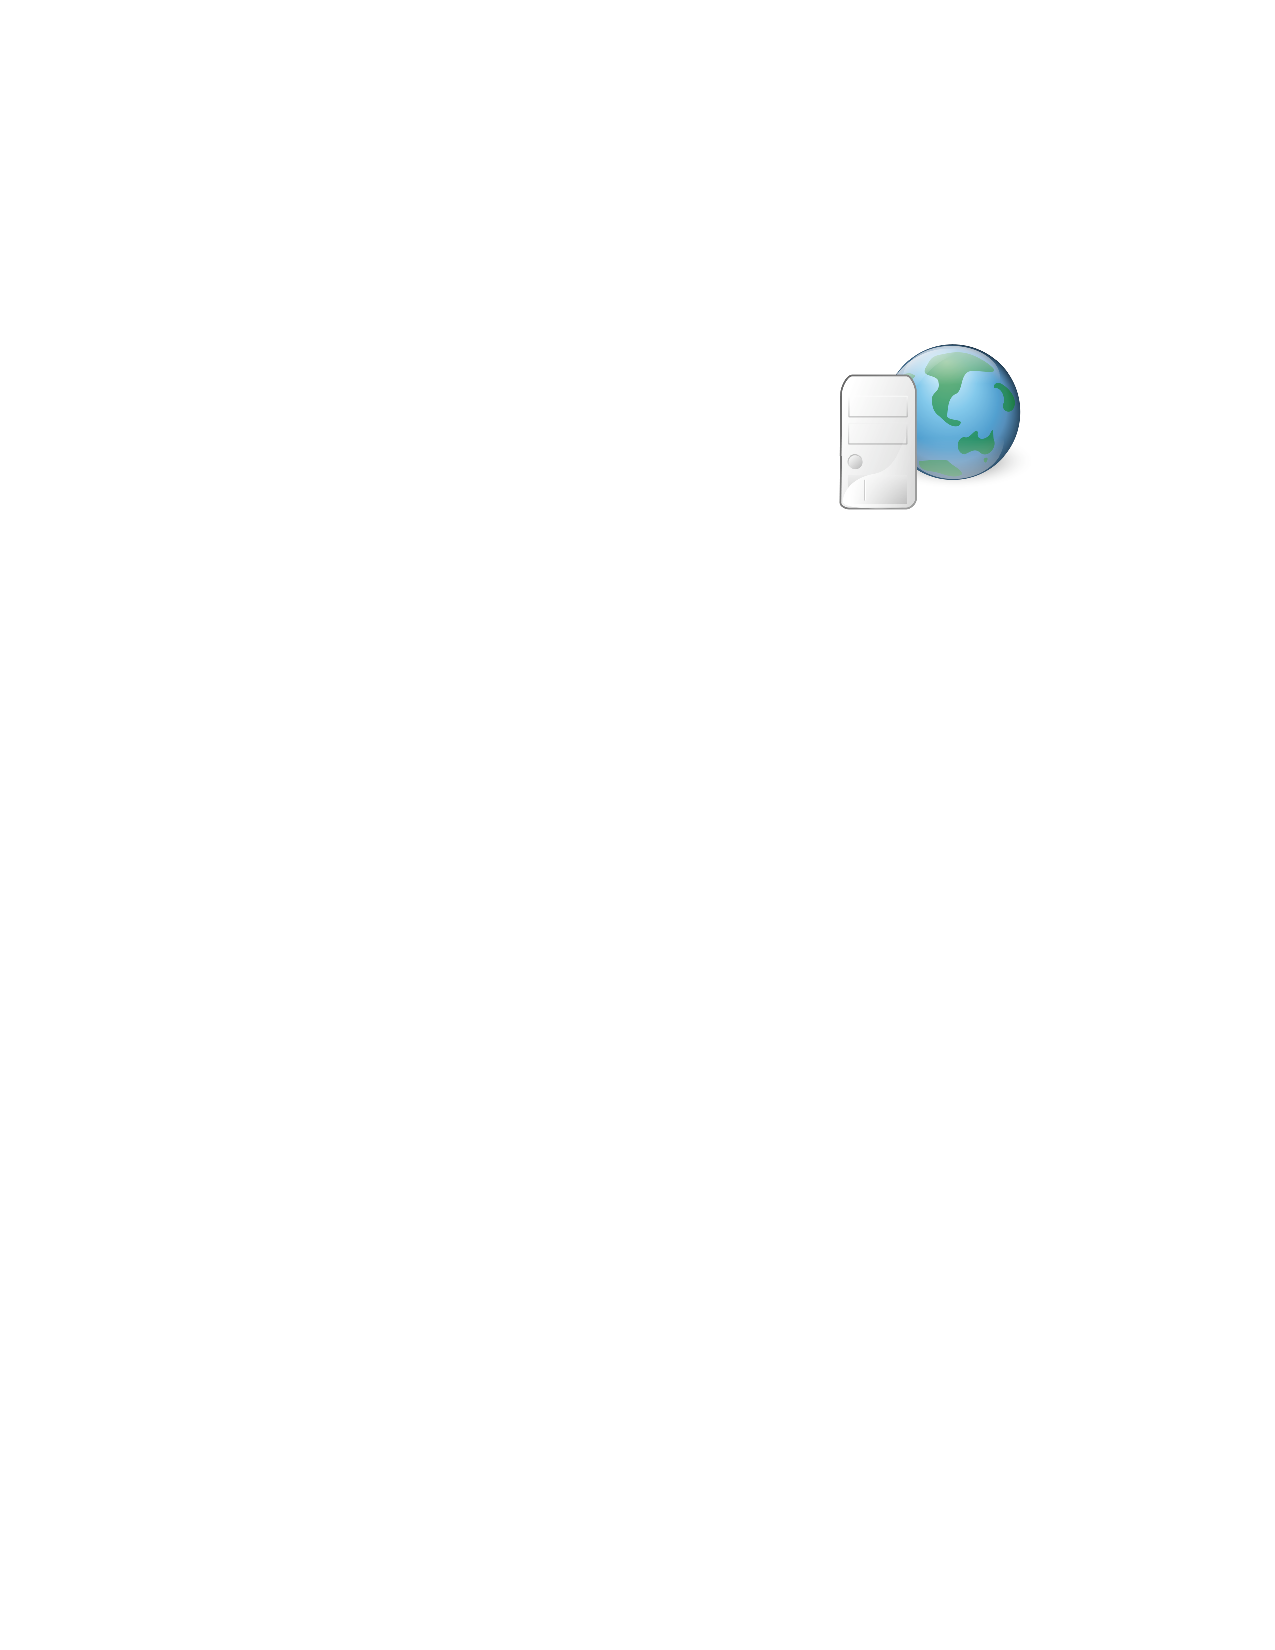
\includegraphics[width=1.5cm]{figures/webserver}};
		\node[shape=cylinder,draw=httpdcolor,thick,shape border rotate=90,xshift=1.25cm,yshift=-0.25cm,minimum width=1.2cm,fill=httpdcolor,fill opacity=0.5] at (0,0) {};
	\end{scope}
	
	\draw[httpdcolor,very thick,<-,curve to,out=180,in=0] (webserver.west) to node[fill=white,key,draw,cloud,aspect=2] {\parbox{2.5cm}{\centering HTTP Content Distribution Network}} ($(cvmfs.east)+(\gap cm,0)$);
	
	\node[key] (volimage) at (1.75cm,-2.25cm) {\parbox{3cm}{\centering File System Buffers}};
	\node[key] (volcache) at (6.25cm,-2.25cm) {\parbox{3.5cm}{\centering CernVM-FS\\ Hard Disk Cache}};
	\node[key] (volrelease) at (13.25cm,-2.25cm) {\parbox{3.5cm}{\centering CernVM-FS ``Repository''\\ (All Releases Available)}};
	\draw[decorate,decoration={expanding waves,segment length=0.1cm,angle=7}] (volimage.east) -- (volcache.west);
	\draw[decorate,decoration={expanding waves,segment length=0.1cm,angle=7}] (volcache.east) -- (volrelease.west);
	
\end{tikzpicture}

%\end{document}
}
	\end{center}
	\caption{A \cvmfs\ client provides a virtual file system that loads data only on access.  
		In this example, all releases of a sofware package (such as an HEP experiment framework) are hosted as a \cvmfs\ repository on a web server.}
	\label{fig:concept}
\end{figure}

\begin{figure}
	\begin{center}
		%\documentclass[a4paper, 11pt]{article}\usepackage{tikz,ifthen}\usetikzlibrary{arrows,positioning,shapes,topaths,calc,fit,backgrounds,matrix,shadows}\begin{document}

\begin{tikzpicture}
	[block/.style={node distance=0.5cm,draw,minimum height=0.7cm,font=\footnotesize,minimum width=3cm},
	 fig/.style={}]
	 
	 \colorlet{cvmfscolor}{green!50!black}
	
	\node[block] (open) at (0,0) {\texttt{open(/ChangeLog)}};
	\node[block] (glibc) [below = of open] {glibc};
	
	\node[block, minimum height=2.5cm,yshift=-1cm] (vfs) [below = of glibc] {\parbox{2.5cm}{\centering VFS\\inode cache\\dentry cache}};
	\node[block, minimum height=1cm,yshift=0.25cm] (buffer cache) [below = of vfs] {\parbox{2.5cm}{\centering Buffer cache}};
	\node[block] (ext3) [right = of buffer cache.south east,yshift=0.35cm,xshift=0.5cm] {ext3};
	\node[block] (NFS) [above = of ext3] {NFS};
	\node (dots) [node distance=0,above = of NFS,yshift=0.3cm] {$\vdots$};
	\node[block] (Fuse) [above = of NFS,yshift=0.6cm] {Fuse};
	\node (vfsv) [left = of Fuse] {};
	
	\node[block] (libfuse) [right = of glibc, xshift=0.5cm] {libfuse};
	\node[block, cvmfscolor, very thick] (cvmfs) [above = of libfuse] {CernVM-FS};
	
	\node[fig] (sqlite) [right = of cvmfs,xshift=1cm,yshift=-1.25cm] {\includegraphics[width=1cm]{figures/memcache} 
\includegraphics[width=2.5cm]{figures/sqlite}};
	\node[fig] (cache) [right = of cvmfs,xshift=1cm,yshift=0.5cm] {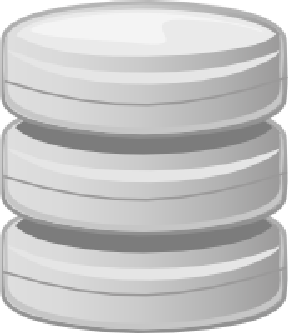
\includegraphics[width=1cm]{figures/cache}};
	\node[fig] (webserver) [right = of cache,yshift=1.5cm] {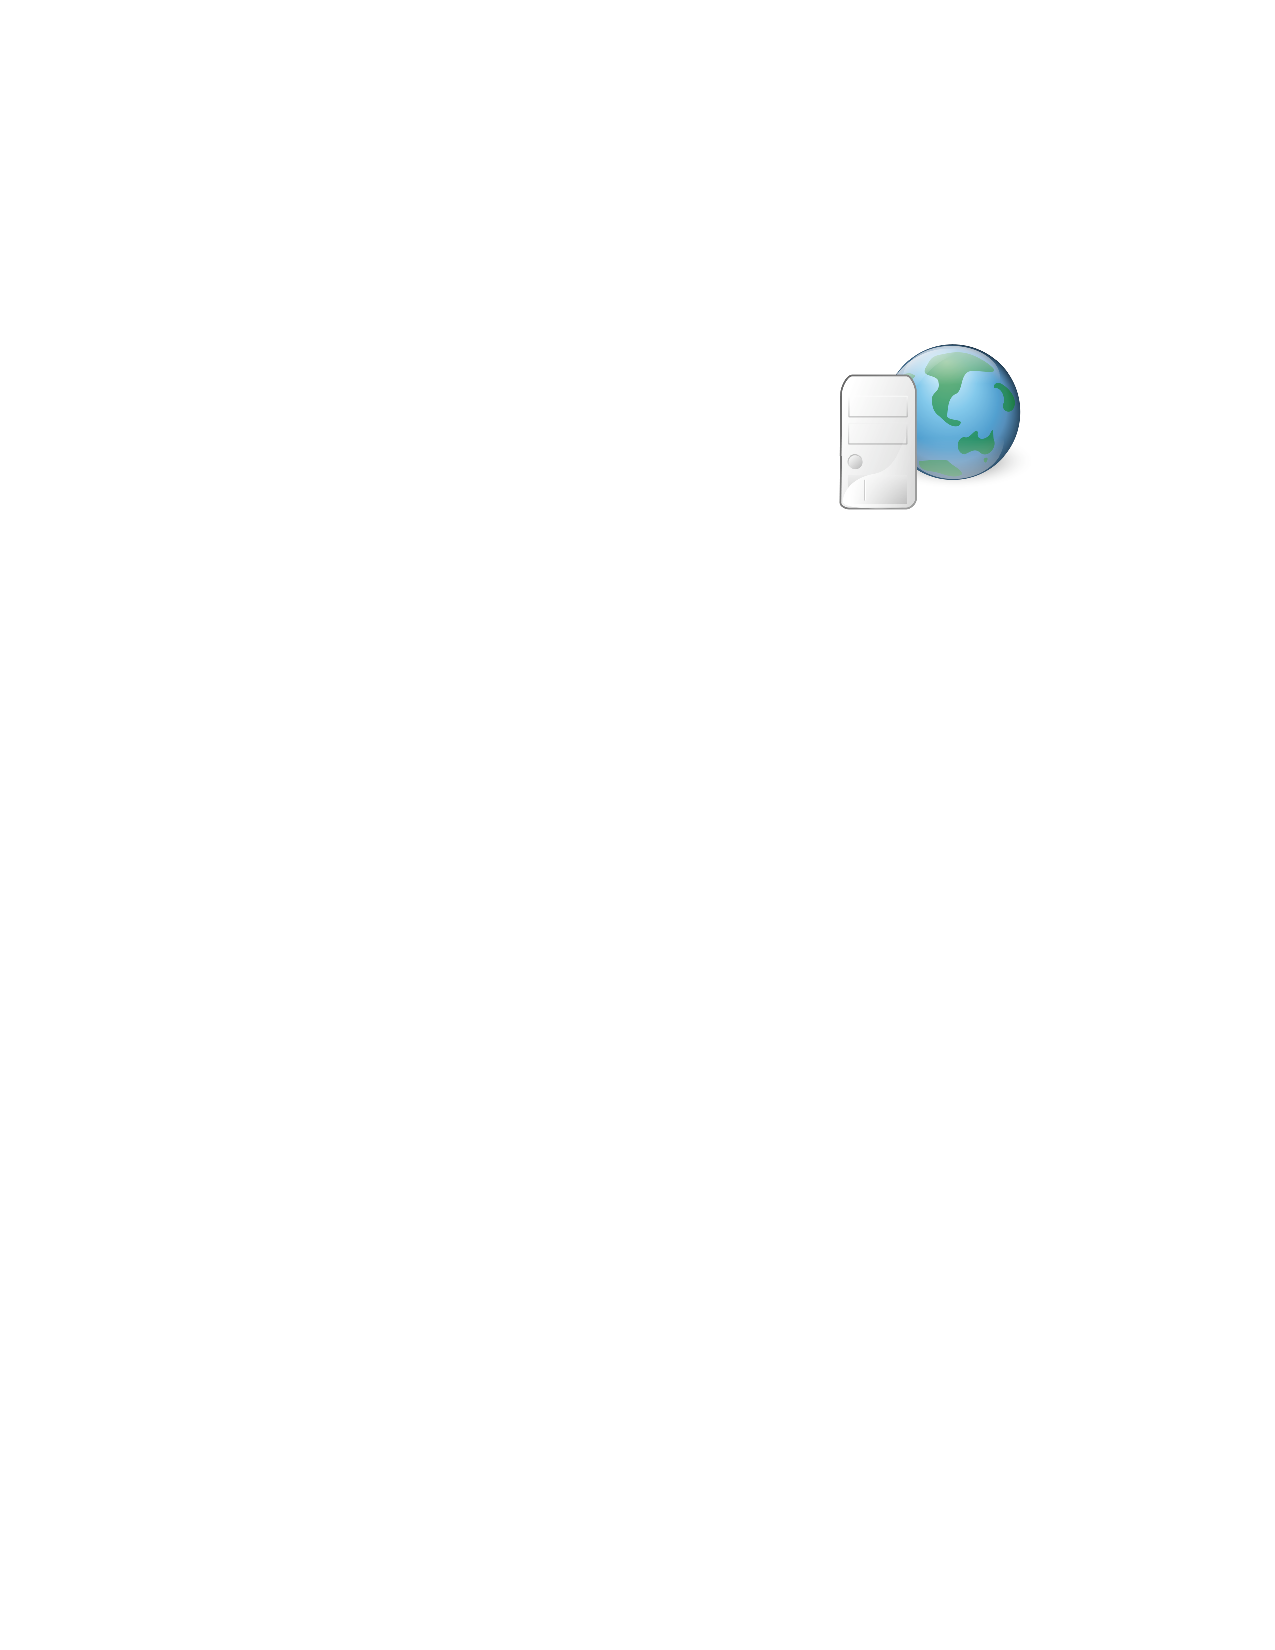
\includegraphics[width=2cm]{figures/webserver}};
	
	\node[node distance=0.8cm] (splitleft) [below=of glibc,xshift=-2cm] {};
	\node[node distance=0.8cm] (splitright) [below=of glibc,xshift=+12cm] {};
	\draw[dashed,blue] (splitleft) -- node[blue,above,very near end,anchor=south west] {\footnotesize user space} node[blue,below,very near end,anchor=north west] {\footnotesize kernel space} (splitright);
	
	\draw[->] (open) -- (glibc);
	\draw[->] (glibc) -- node[fill=white,yshift=-1ex] {\footnotesize  syscall} (vfs);
	\draw[->] (vfsv) -- (Fuse);
	\draw[->] (Fuse) -- node[fill=white,yshift=-1ex] {\footnotesize\tt  /dev/fuse} (libfuse);
	\draw[->] (libfuse) -- (cvmfs);
	
	%\draw[->,curve to,out=300,in=200] (cvmfs.south east) to node {} (sqlite.south west) {};
	\draw[->,very thick,cvmfscolor,curve to,out=180,in=10] (sqlite.west) to node [fill=white] {\footnotesize SHA1} (cvmfs.south east) {};
	\draw[<-,very thick,cvmfscolor] (cvmfs.east) -- node[fill=white] {\footnotesize file descr.} (cache.west) {};
	\draw[->, dashed] (cvmfs.west) -- node[above] {\footnotesize fd} (open.east) {};
	\draw[->,very thick,orange,curve to,out=-40,in=-140] (cache.east) to node [near start, right=0.01cm, fill=white] {\footnotesize HTTP GET} (webserver.south west) {};
	\draw[->,very thick,orange,curve to,out=160,in=40] (webserver.west) to node [near start, left=0.01cm, fill=white] {\footnotesize inflate+verify} (cache.north east) {};

	%\draw[<->, dashed, gray, curve to, out=-45,in=20] (cache.south east) to node {} (ext3.east) {};
	
\end{tikzpicture} 

%\end{document}

	\end{center}
	\caption{Opening a file on \cvmfs. \cvmfs\ resolves the name by means of an SQLite catalog, which is prepended by a memory cache. 
		Downloaded files are verified against the cryptographic hash of the corresponding catalog entry. 
		The \texttt{read()} and the \texttt{stat()} system call can be entirely served from the in-kernel file system buffers.}
	\label{fig:fuse}
\end{figure}
